\begin{figure}[t]
\centering
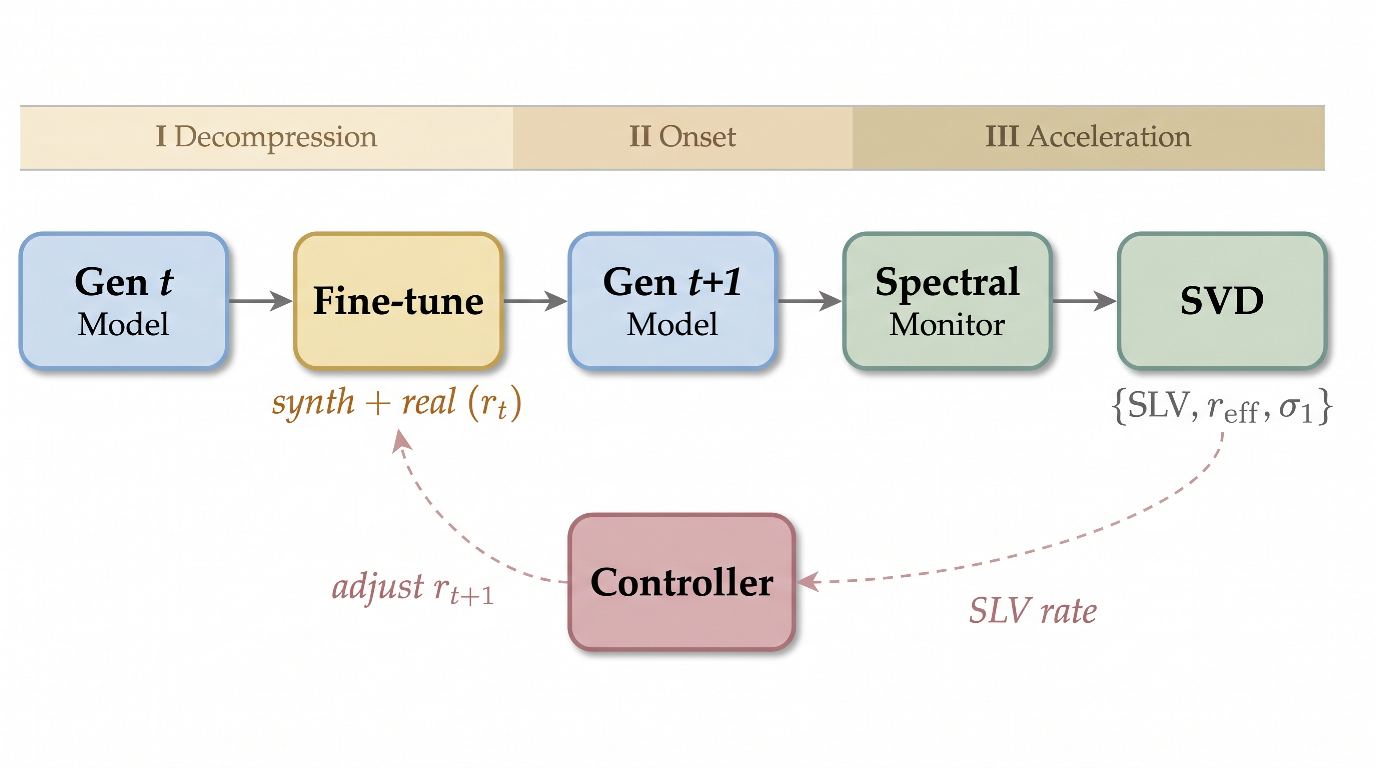
\includegraphics[width=\columnwidth]{figures/pipeline_overview.pdf}
\caption{Experimental pipeline. Each generation fine-tunes on synthetic text mixed with real data at ratio $r_t$. Spectral monitoring extracts last-layer embeddings from held-out data, computes a singular value decomposition (SVD), and derives SLV, $r_{\text{eff}}$, and $\sigma_1$. A proportional controller (dashed) can adjust $r_{t+1}$ based on the SLV rate of change. The three phases (decompression (I), onset (II), and acceleration (III)) are annotated along the generation axis.}
\label{fig:pipeline}
\end{figure}

\paragraph{Model Collapse.}
\citet{shumailov2024collapse} showed that recursive training on model-generated data progressively erodes distributional tails (\emph{model collapse}).
Scaling laws predict tail erosion as a function of recursive depth~\citep{dohmatob2024tails, dohmatob2024demystified, seddik2024synthetic}; the self-consuming loop accelerates collapse even under data accumulation~\citep{alemohammad2024mad}, with as little as 1\% synthetic contamination sufficing~\citep{dohmatob2025strong}, though preserving all prior data can delay it~\citep{gerstgrasser2024inevitable}; mitigations include self-verification~\citep{fu2025selfverification} and weak non-synthetic data~\citep{amin2025escaping}.
Distribution divergence measures (KL divergence, maximum mean discrepancy) offer another detection path but require a reference distribution and do not reveal the geometric structure of collapse.
We complement these output-based diagnoses by tracking collapse through the spectral geometry of internal representations.

\paragraph{Spectral Analysis of Representations.}
Random matrix theory reveals implicit regularization in neural network eigenspectra~\citep{martin2021implicit}; effective rank~\citep{roy2007effectiverank} and RankMe~\citep{rankme2023} quantify representational dimensionality.
\citet{he2025spectral} linked spectral collapse to plasticity loss in continual learning, and \citet{naderi2025mindgap} identified rank collapse in attention matrices.
Most directly relevant, \citet{gu2026sigma} proposed SIGMA, tracking singular-value distributions during recursive training on OPT-125M over three generations.
Our SLV equals half of SIGMA's $\log\det G$; we extend SIGMA in \emph{scale} (Pythia-410M/1B, 3--8$\times$ larger), \emph{temporal depth} (10 vs.\ 3 generations), and \emph{methodology} (SLV-based mixing control).
Table~\ref{tab:related_comparison} summarizes the positioning.

\paragraph{Early Warning Signals and Critical Transitions.}
EWS for critical transitions originate in ecology, where rising autocorrelation and variance precede regime shifts~\citep{scheffer2009ews, scheffer2012anticipating}, with methods from statistical tests~\citep{dakos2012methods} to deep learning~\citep{bury2021deeplearning}.
A central tension is that stabilization interventions suppress the precursors they rely on~\citep{scheffer2009ews}; we encounter a stronger form where real-data mixing reverses the spectral trajectory entirely (\S\ref{subsec:controller}).

\paragraph{Data Mixing for LLM Training.}
Data composition significantly affects LM quality~\citep{longpre2024pretrainer, muennighoff2023scaling}, and several methods optimize domain mixtures~\citep{xie2023doremi, ye2025mixinglaws, chen2025aioli}, but evaluate mixing through loss or benchmarks.
Our work reveals that real-vs-synthetic mixing reshapes the spectral geometry of representations, producing a trajectory map that loss-based metrics do not capture.

\begin{table}[t]
\centering
\small
\setlength{\tabcolsep}{3pt}
\begin{tabular}{@{}lccc@{}}
\toprule
& \textbf{SIGMA} & \textbf{He+ '25} & \textbf{This work} \\
\midrule
Setting & Recursive & Continual & Recursive \\
Scale & 125M & Various & 410M + 1B (pilot) \\
Generations & 3 & --- & 10 \\
Spectral metric & $\log\det G$ & spec.\ norm & SLV \\
Phase typology & --- & --- & \checkmark \\
Mixing / $r_{\text{crit}}$ & --- & --- & \checkmark \\
Controller & --- & --- & \checkmark \\
\bottomrule
\end{tabular}
\caption{Positioning relative to recent spectral-collapse studies. SLV $\equiv \tfrac{1}{2}\log\det G$. SIGMA: \citet{gu2026sigma}; He+: \citet{he2025spectral}.}
\label{tab:related_comparison}
\end{table}
